\chapter{PLL Integration}
Model the PLL loop, choose \(K_{VCO}\), set loop bandwidth and stability, and budget total jitter. Interactions among PFD/CP/LF and the \VCO{} control dictate spur and phase-noise transfer.

\section{Integer-$N$ PLL Model}
Let the PFD gain be \(K_{\mathrm{PFD}}=\pm 1\,\mathrm{A/rad}\), charge pump current \(I_{\mathrm{CP}}\), loop filter transfer \(Z(s)\), divider ratio \(N\), and VCO gain \(K_{VCO}\,[\mathrm{Hz/V}]\). The open-loop transfer is
\[
 L(s) = \frac{K_{\mathrm{PFD}}\,I_{\mathrm{CP}}\,Z(s)\,K_{VCO}}{s\,N}
\]
The closed-loop phase transfer from reference to output is
\[
 H_{ref\to out}(s) = \frac{L(s)}{1+L(s)}\,,\quad H_{vco\,noise}(s) = \frac{1}{1+L(s)}
\]
so the PLL suppresses VCO phase noise inside the loop bandwidth and tracks the reference; the opposite occurs outside.

\section{Type-II, Second-Order Example}
With a standard R\,C filter (zero at \(\omega_z\), pole at origin), the unity gain frequency (UGF) \(\omega_c\) and phase margin \(\phi_m\) are tuned by \(R\) and \(C\). A practical target is \(\phi_m\approx 55^\circ\)–\(65^\circ\) and \(\omega_c \approx f_{ref}/10\) to limit reference spurs.

\begin{figure}[H]
  \centering
  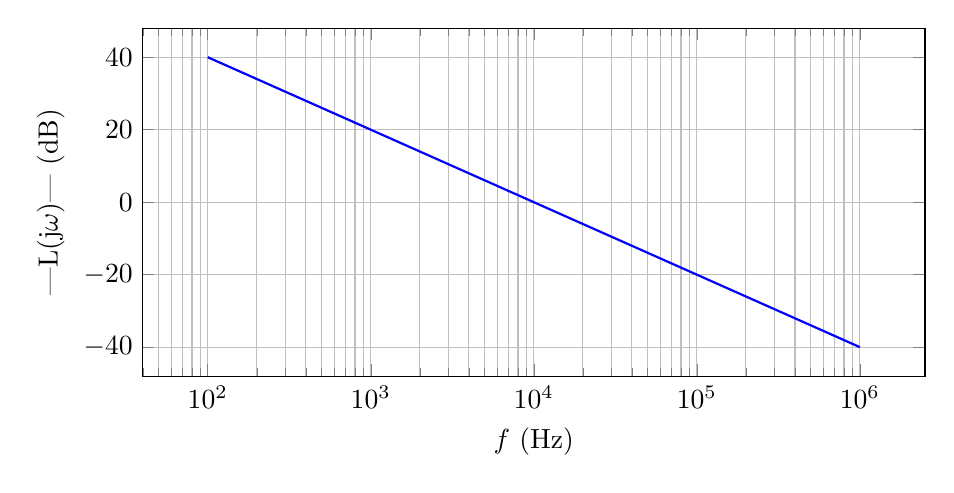
\begin{tikzpicture}
    \begin{axis}[width=0.95\linewidth, height=6cm, xmode=log, grid=both, xlabel={$f$ (Hz)}, ylabel={|L(j$\omega$)| (dB)}]
      \addplot[blue, thick] table[row sep=\\]{x y \\
        1e2  40 \\
        1e3  20 \\
        1e4   0 \\
        1e5 -20 \\
        1e6 -40 \\
      };
    \end{axis}
  \end{tikzpicture}
  \caption{Illustrative open-loop magnitude |L(j$\omega$)| with Type-II loop}
\end{figure}

\section{Noise and Spur Transfer}
The output phase-noise PSD is
\[
 S_{\phi\phi,\,out}(f) \approx |H_{ref\to out}(j2\pi f)|^2 S_{\phi\phi,\,ref}(f) + |H_{vco\,noise}(j2\pi f)|^2 S_{\phi\phi,\,vco}(f) + S_{LF}(f)
\]
where \(S_{LF}\) accounts for loop-filter resistor noise and CP noise shaped by the loop. Reference spurs at \(\pm f_{ref}\) arise from charge pump ripple leaking through \(Z(s)\); mitigate by increasing attenuation at \(f_{ref}\) or using active filters/scrambling.

\section{Fractional-$N$ Considerations}
Sigma–delta modulation of the divider introduces quantization noise shaped to high offset; ensure the loop bandwidth is set to suppress in-band noise and randomize modulator to avoid tonal spurs. DCO/varactor banks should be scrambled or DEMed to reduce mismatch-induced tones.

\section{Jitter Budget}
Allocate RMS jitter contributions by root-sum-of-squares (RSS): reference, PFD/CP, loop filter, divider, VCO (residual outside bandwidth). A typical budget dedicates 50–70\% to VCO far-out, 20–30\% to in-band electronics, and the rest to reference.

\section{Block Diagram}
\begin{figure}[H]
  \centering
  \begin{tikzpicture}[node distance=1.5cm, >=Latex]
    \tikzstyle{blk}=[draw, rounded corners, minimum width=2.6cm, minimum height=0.9cm]
    \node[blk] (ref) {Reference};
    \node[blk, right=of ref] (pfd) {PFD/CP};
    \node[blk, right=of pfd] (lf) {Loop Filter $Z(s)$};
    \node[blk, right=of lf] (vco) {VCO $K_{VCO}$};
    \node[blk, below=1.2cm of vco] (div) {Divider $N$};
    \draw[->] (ref) -- (pfd);
    \draw[->] (pfd) -- (lf);
    \draw[->] (lf) -- (vco);
    \draw[->] (vco) -- ++(1.0,0) node[right] {$\phi_{out}$};
    \draw[->] (vco) |- (div);
    \draw[->] (div) -| (pfd);
  \end{tikzpicture}
  \caption{PLL with PFD/CP, loop filter, VCO, and feedback divider}
\end{figure}

\section{Design Targets and Parameters}
\begin{table}[H]
  \centering
  \begin{tabular}{lll}
    \toprule
    Parameter & Target & Note \\
    \midrule
    Reference $f_{ref}$ & 1 MHz & crystal source \\
    Divider $N$ & 10 & $f_0=10$ MHz \\
    UGF $\omega_c/2\pi$ & 100 kHz & $\approx f_{ref}/10$ \\
    Phase margin $\phi_m$ & $60^\circ$ & stability reserve \\
    $K_{VCO}$ & 1–3 MHz/V & from Ch.~5 sizing \\
    CP current $I_{CP}$ & 50–200 $\mu$A & spur vs bandwidth trade-off \\
    \bottomrule
  \end{tabular}
  \caption{Illustrative PLL design parameters}
\end{table}

\section{Reference Spur Mapping}
\begin{figure}[H]
  \centering
  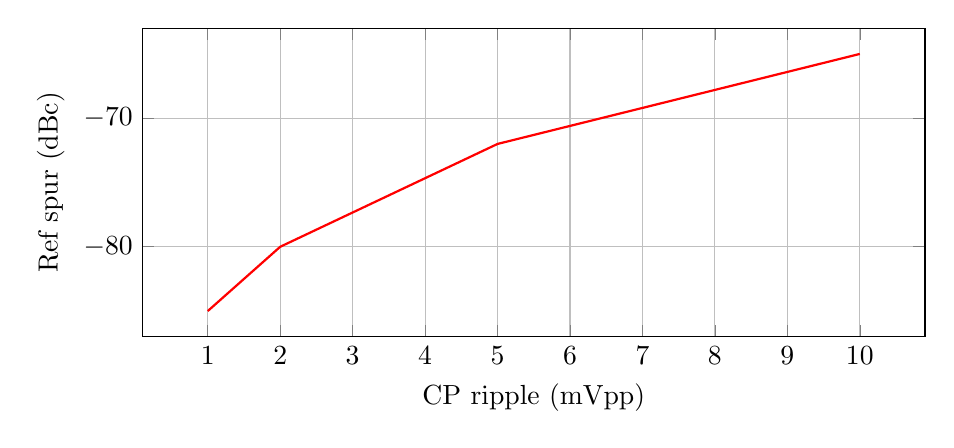
\begin{tikzpicture}
    \begin{axis}[
      width=0.95\linewidth, height=5.5cm,
      xlabel={CP ripple (mVpp)}, ylabel={Ref spur (dBc)}, grid=both]
      \addplot[red, thick] table[row sep=\\]{x y \\
        1   -85 \\
        2   -80 \\
        5   -72 \\
        10  -65 \\
      };
    \end{axis}
  \end{tikzpicture}
  \caption{Illustrative reference spur level vs. charge-pump ripple}
\end{figure}


